\documentclass[tikz,border=2pt,11pt]{standalone}
\usetikzlibrary{calc}
\usetikzlibrary{arrows.meta}
\usetikzlibrary{positioning}
\usepackage{amsmath}
\usepackage{amssymb}
\usepackage{mathrsfs}
\usepackage{graphicx}
\usepackage{xcolor}
\usepackage{tikz}
\newcommand{\DoNotLoadEpstopdf}{}
\newcommand{\Fp}{\mathbf F_p}
\newcommand{\Fq}{\mathbf F_q}
\newcommand{\Z}{\mathbf Z}
\newcommand{\Q}{\mathbf Q}
\newcommand{\C}{\mathbf C}
\DeclareMathOperator{\Gal}{Gal}
\DeclareMathOperator{\Pic}{Pic}
\DeclareMathOperator{\Tr}{Tr}
\DeclareMathOperator{\Nm}{N}
\DeclareMathOperator{\End}{End}
\DeclareMathOperator{\Hom}{Hom}
\DeclareMathOperator{\ord}{ord}
\DeclareMathOperator{\divisor}{div}
\DeclareMathOperator{\Spec}{Spec}
\DeclareMathOperator{\im}{im}
\begin{document}
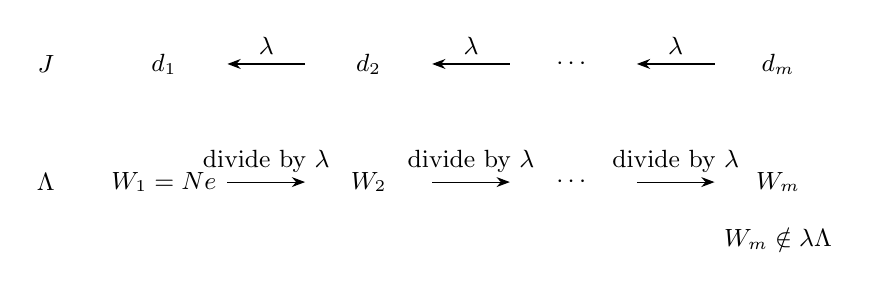
\begin{tikzpicture}[>=Stealth, every node/.style={font=\small},
                    point/.style={minimum width=1.6cm,minimum height=0.7cm}]
 \node at (-1.5,0) {$J$};
 \node at (-1.5,-1.5) {$\Lambda$};
 \node[point] (d1) at (0,0) {$d_1$};
 \node[point] (d2) at (2.6,0) {$d_2$};
 \node[point] (dd) at (5.2,0) {$\cdots$};
 \node[point] (dm) at (7.8,0) {$d_m$};
 \draw[->] (d2) -- node[above] {$\lambda$} (d1);
 \draw[->] (dd) -- node[above] {$\lambda$} (d2);
 \draw[->] (dm) -- node[above] {$\lambda$} (dd);
 \node[point] (w1) at (0,-1.5) {$W_1=Ne$};
 \node[point] (w2) at (2.6,-1.5) {$W_2$};
 \node[point] (ww) at (5.2,-1.5) {$\cdots$};
 \node[point] (wm) at (7.8,-1.5) {$W_m$};
 \draw[->] (w1) -- node[above] {divide by $\lambda$} (w2);
 \draw[->] (w2) -- node[above] {divide by $\lambda$} (ww);
 \draw[->] (ww) -- node[above] {divide by $\lambda$} (wm);
 \node[below=1mm of wm] {$W_m\notin\lambda\Lambda$};
\end{tikzpicture}
\end{document}
